\section{Gestion des permissions}

\textbf{Si vous êtes un admin}, vous pouvez alors accéder à la page de gestion des permissions, depuis l'onglet "Staff" tout à droite du menu de navigation.

\begin{figure}[H]
\centering
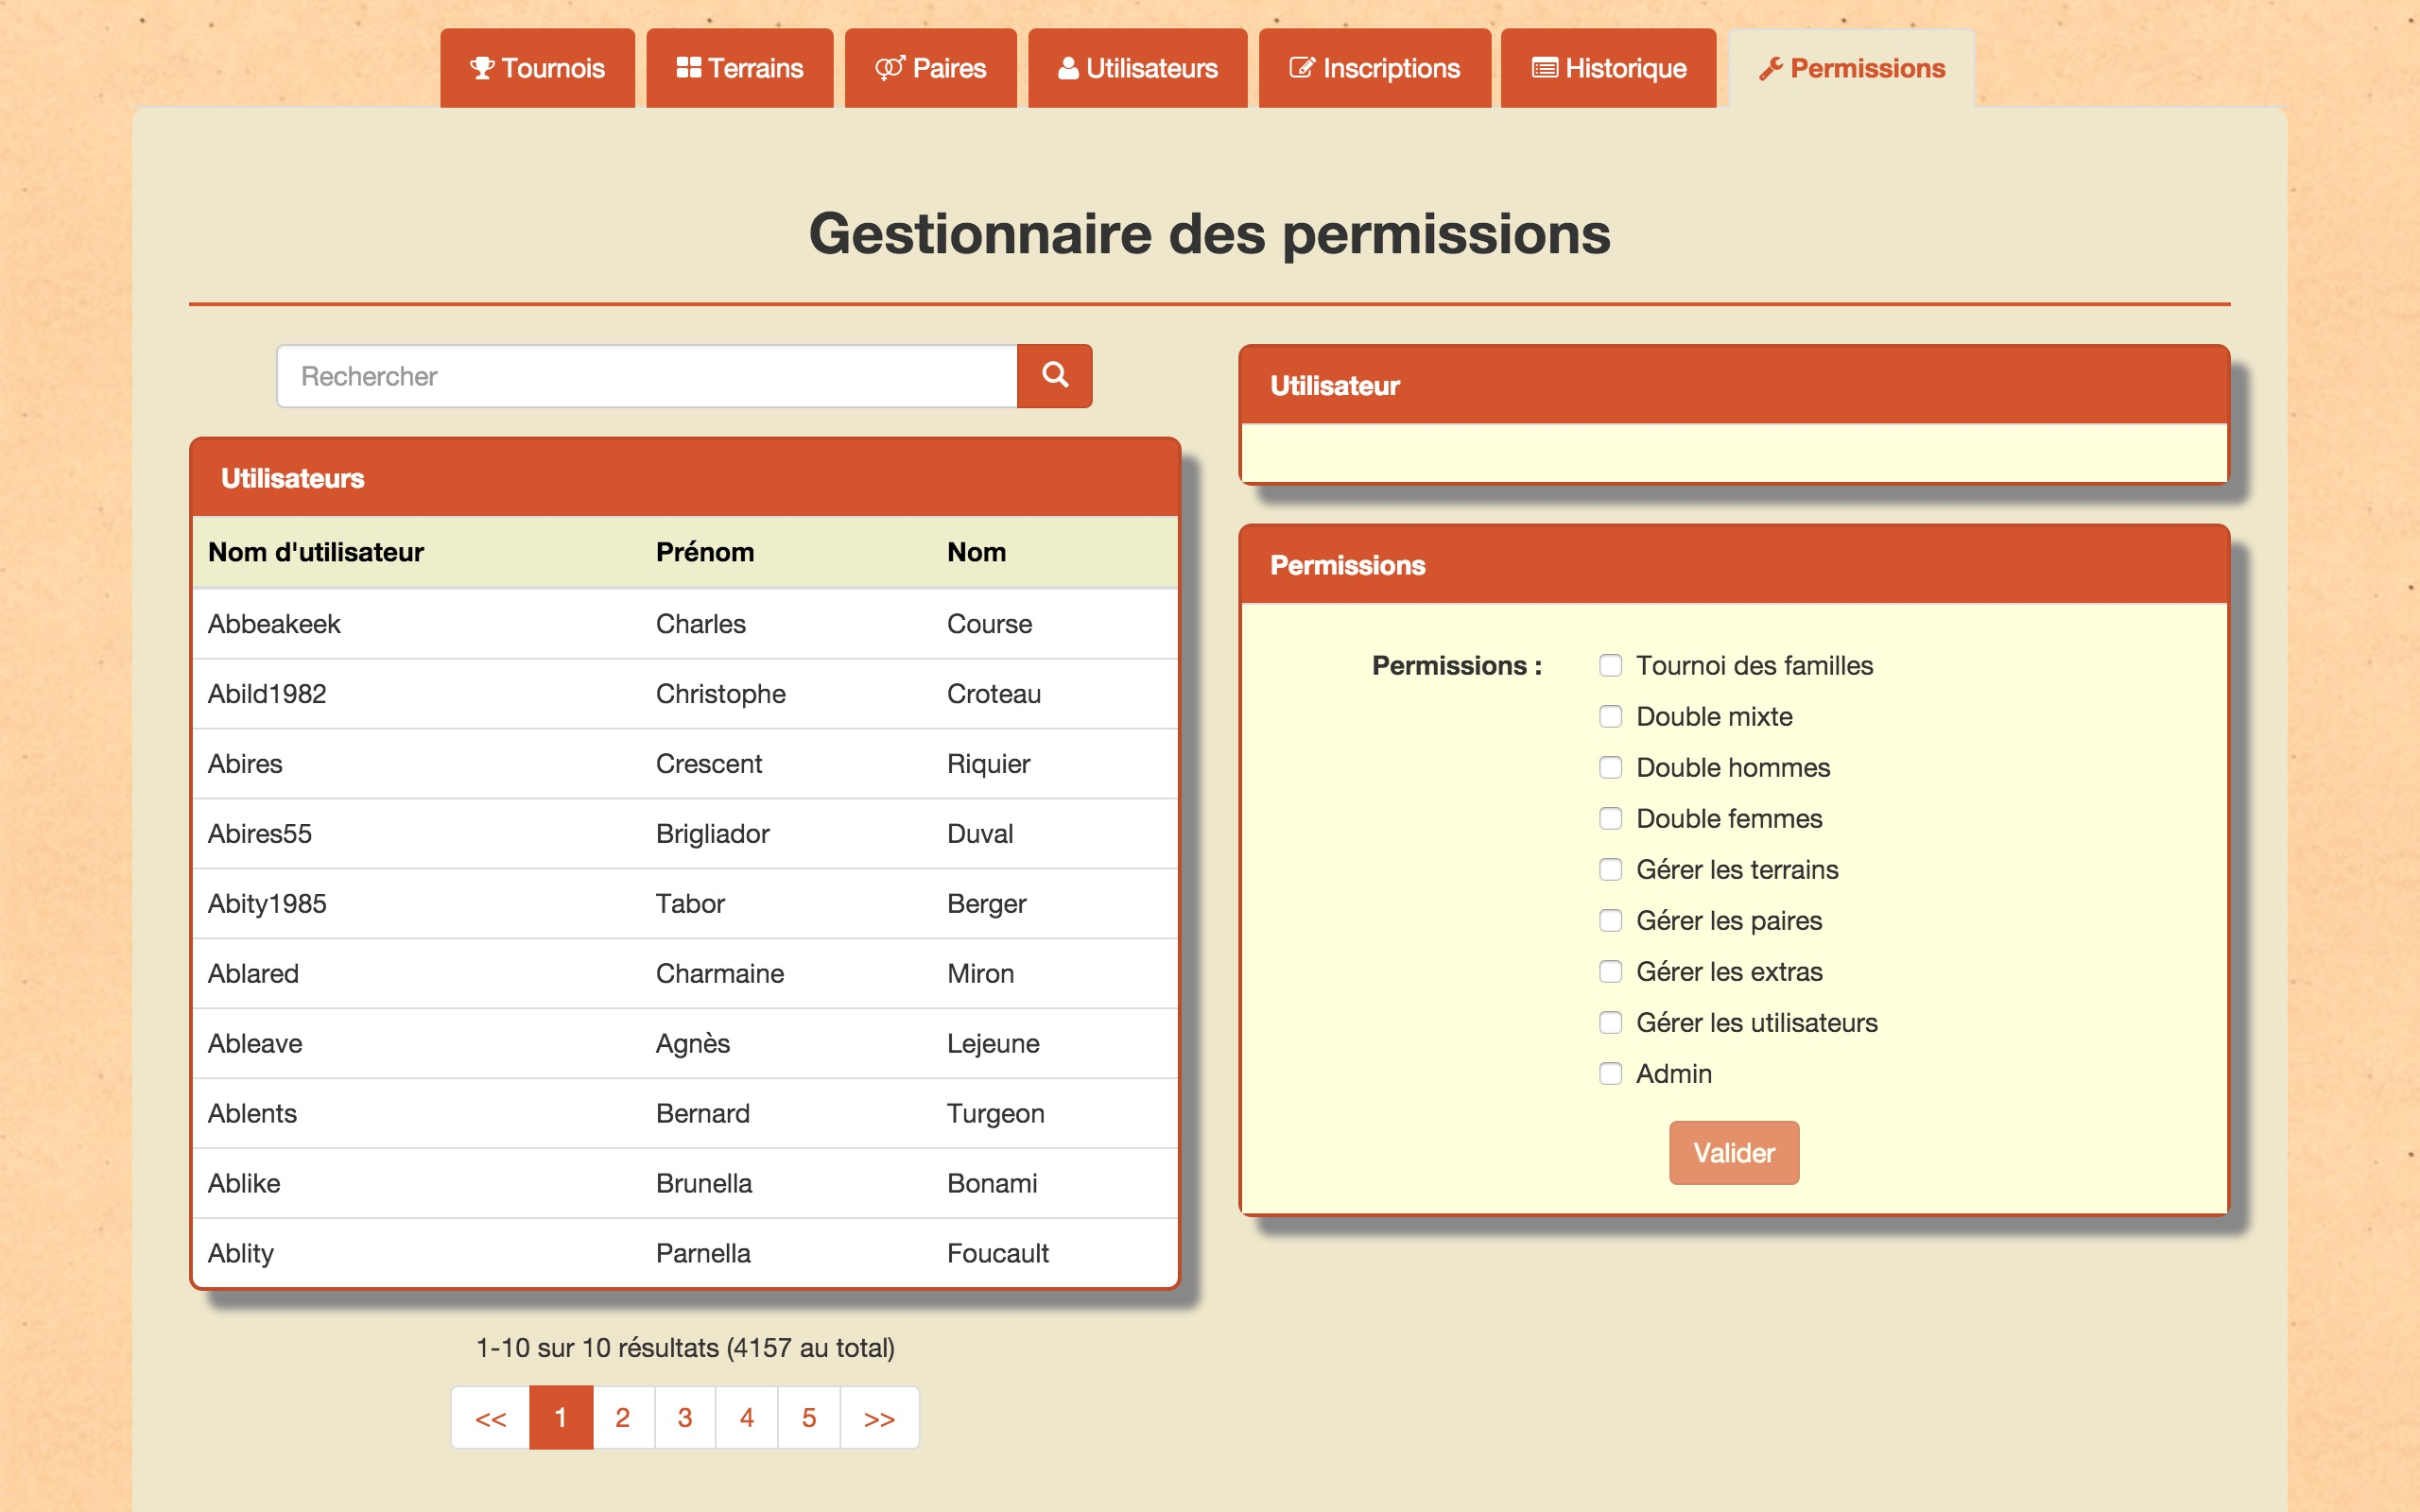
\includegraphics[scale=0.15]{gestion-permissions/gestion-permissions.jpg}
\caption{Page admin pour la gestion des permissions}
\end{figure}

Cette page permet de modifier les permissions des utilisateurs. Elle est divisé en deux parties :

\begin{itemize}
\item  à gauche, un champ de recherche, avec une liste d'utilisateurs ;
\item à droite, une case contenant le nom de l'utilisateur sélectionné, ainsi qu'une liste de permissions à cocher et valider via le bouton \textit{Valider}
\end{itemize}
\bigskip

Pour modifier les permission d'un utilisateur, on sélectionne l'utilisateur dans la liste des utilisateur que l'on souhaite modifier ses permissions, puis on coche ou décoche les permissions voulues, et on applique les changements de permissions en cliquant sur le bouton \textit{Valider}.\newline

\begin{figure}[H]
\centering
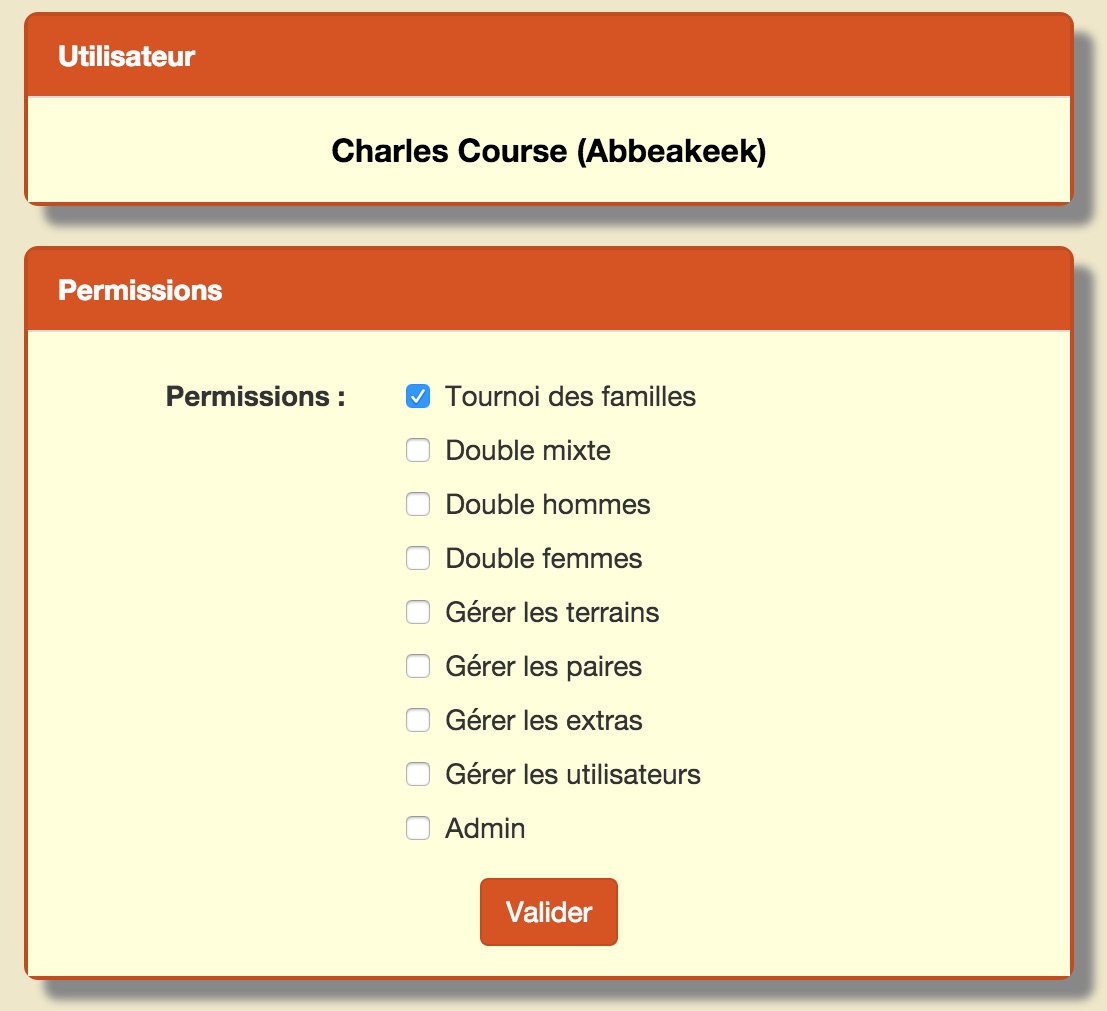
\includegraphics[scale=0.25]{gestion-permissions/gestion-permissions-user.jpg}
\caption{Permission actuel de l'utilisateur "Abbeakeek" sur la page de la gestion des permissions}
\end{figure}

L'utilisateur Abbeakeek dans la liste des utilisateurs a la permission de gérer le tournoi des familles.

\begin{figure}[H]
\centering
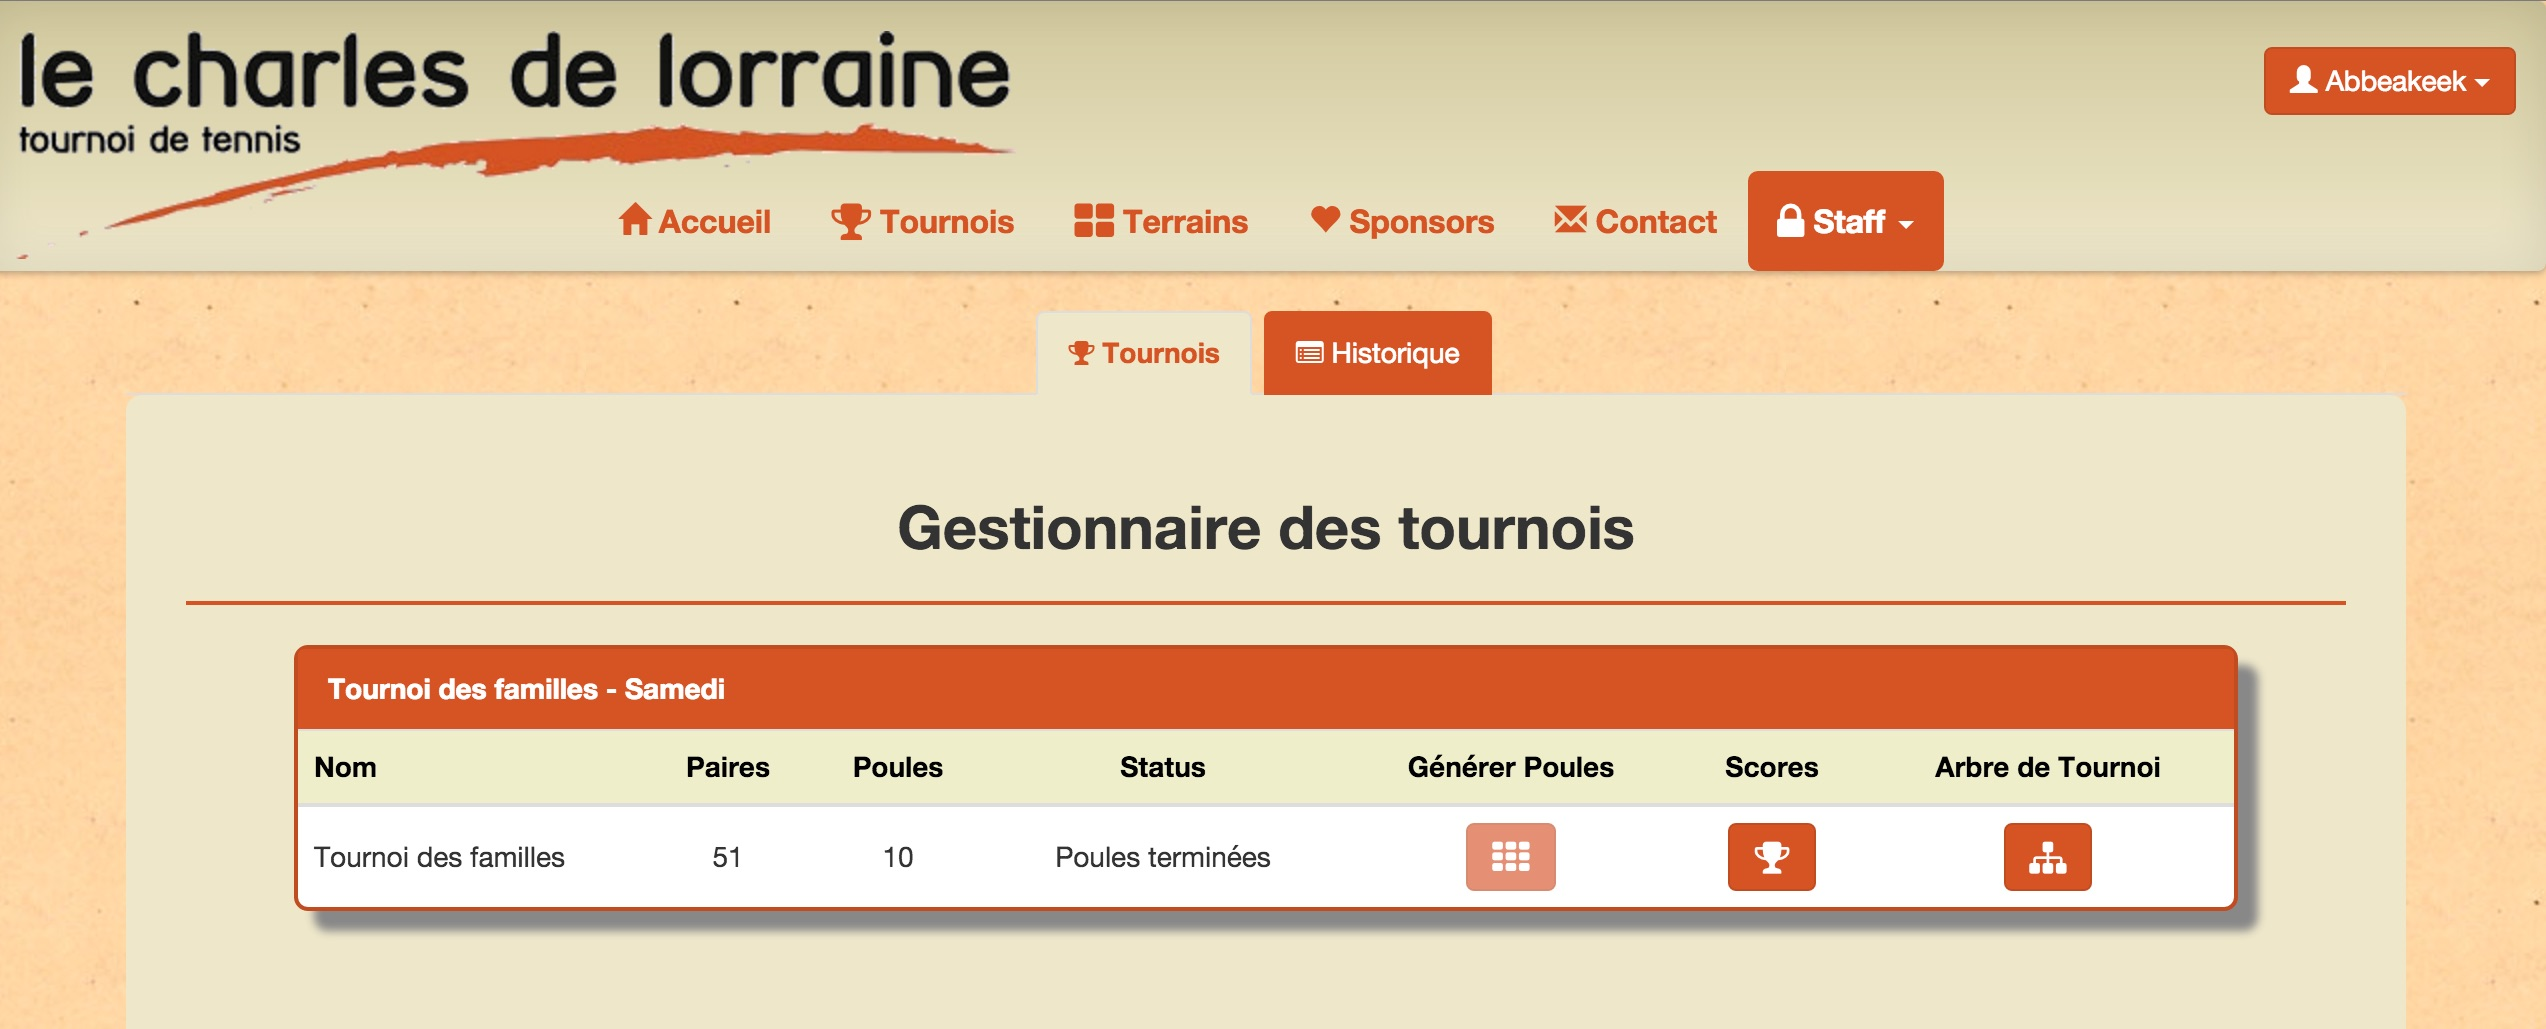
\includegraphics[scale=0.15]{gestion-permissions/gestion-permissions-permission1.jpg}
\caption{Permission actuel de l'utilisateur Abbeakeek - uniquement capable de gérer le tournoi des familles}
\end{figure}

En lui ajoutant la permission de gérer les terrains, il est autorisé à accéder à la page de gestion des terrains.

\begin{figure}[H]
\centering
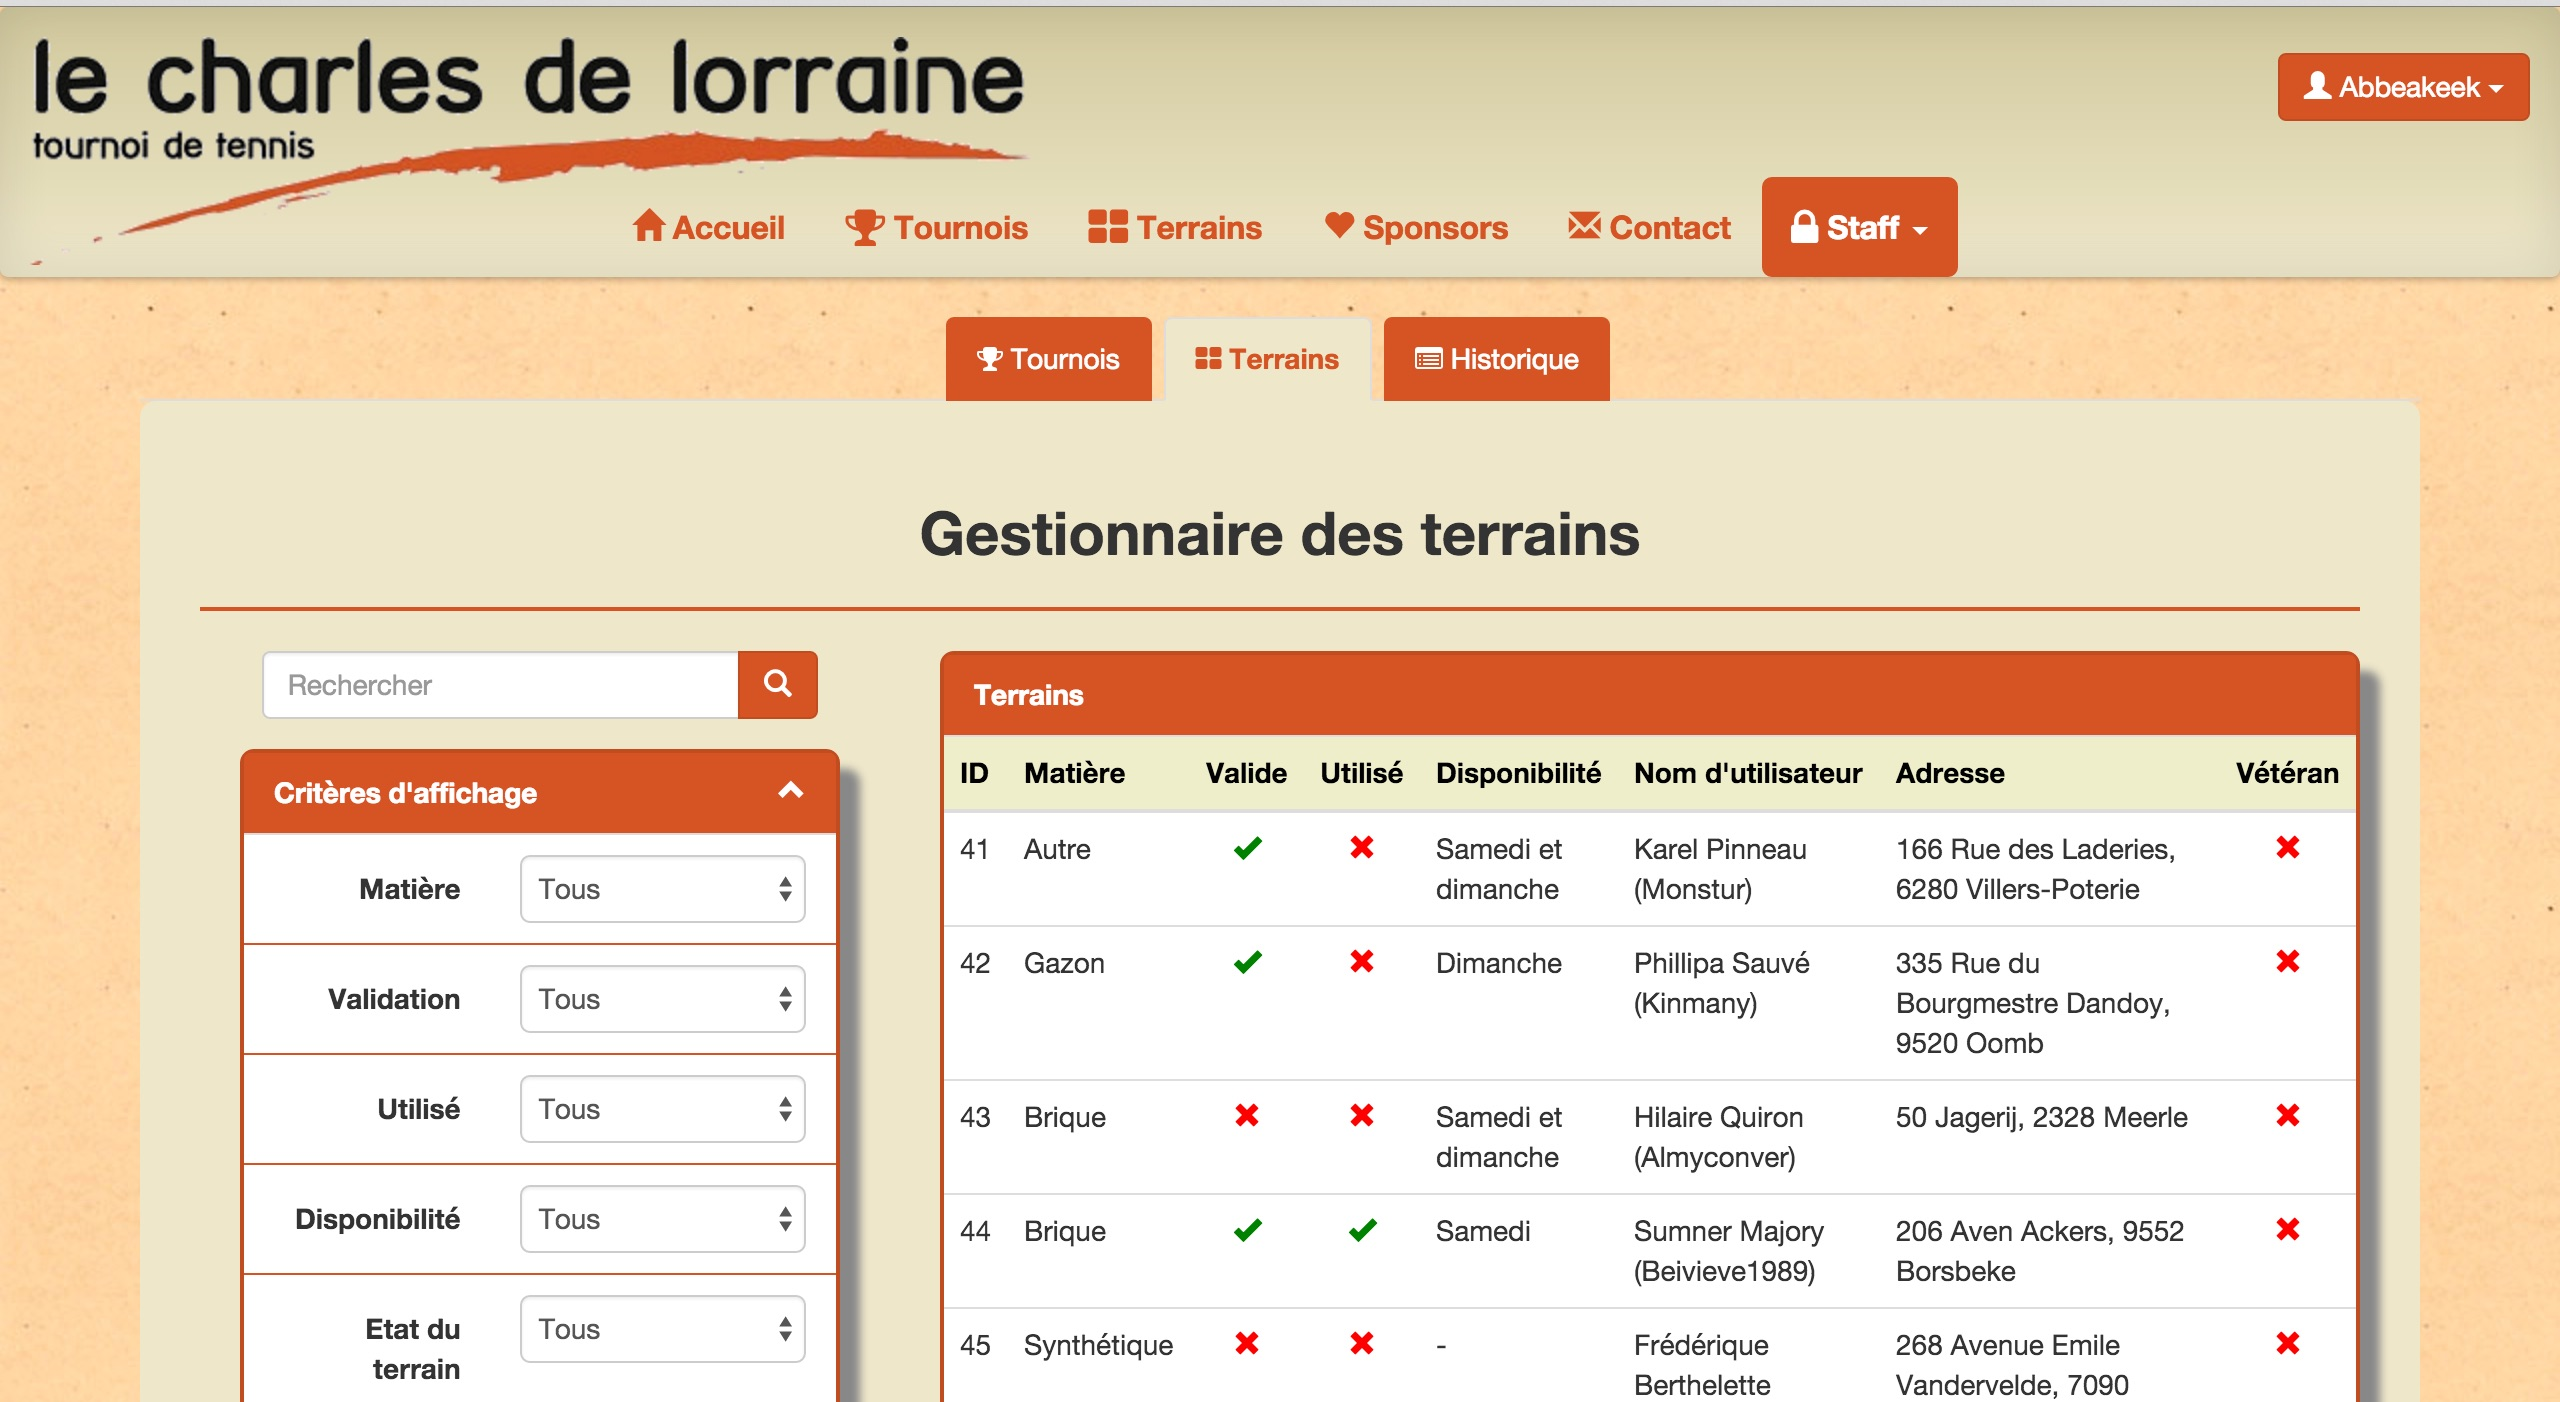
\includegraphics[scale=0.15]{gestion-permissions/gestion-permissions-permission2.jpg}
\caption{Nouvelle permission de l'utilisateur Abbeakeek - capable de gérer les terrains}
\end{figure}
